\chapter{Task 2}\label{chapter:introduction}

\section{Jacobian matrix compression}
\label{sec:jacobian-matrix-compression}


The main goal of Jacobian matrix compression is minimization of the number of non-linear function evaluations which is a quite compute-intensive operation. Minimization is performed by means of efficient treatment of non-zero entries due to matrix sparsity. The problem is also known as matrix partitioning.\\


In the general case, finite difference method can be used to compute a Jacobian matrix approximation in the following way:\\

\begin{equation} \label{eq:matrix-compression-1}
	\frac{1}{\epsilon} (F(y + \epsilon e_{k}) - F(y)) \approx J(y) e_{k}, \: \: \: 1 \leq k \leq N
\end{equation}

where $F : \mathbb{R}^{N} \rightarrow \mathbb{R}^{N}$  is a non-linear function, $e_{k} \in \mathbb{R}^{N}$ is the k\textit{th} coordinate unit vector, $\epsilon$ is a small step size.\\


Equation \ref{eq:matrix-compression-1} does not exploit Jacobian matrix sparsity and, therefore, estimation of a Jacobian matrix requires $N$  function evaluations.\\


\figpointer{\ref{fig:example-of-matrix-compression}}
\begin{figure}[htpb]
  \centering
  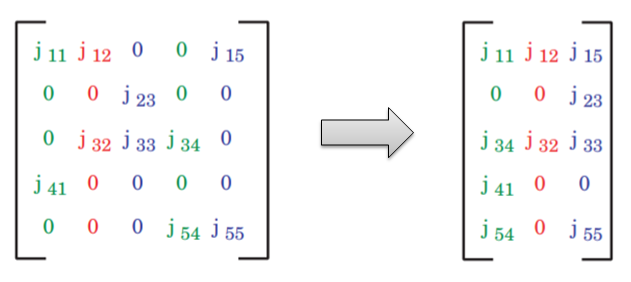
\includegraphics[width=0.55\textwidth]{figures/chapter-3/matrix-compression-example.png}
\caption{An example of matrix coloring and compression \cite{gebremedhin2005color}}
\label{fig:example-of-matrix-compression}
\end{figure}


The compression algorithm is based on a notion of \textit{structurally orthogonal} columns i.e. columns which do not share any non-zero entry in a common row. Figure \ref{fig:example-of-matrix-compression} shows an example of matrix compression where each color denotes independent, structurally orthogonal, columns.\\


% Curtis, Powell, and Reid [35] were the first to observe in 1974 that sparsity can be employed in this way to reduce the number of function evaluations needed to estimate the Jacobian.


Having obtained a compressed form of Jacobian, another set of vectors $d \in \mathbb{R}^{N}$, also known as seed vectors, can be used to perform function perturbation in stead of unit vectors $e_{k}$. A seed vector $d$ has 1’s in components corresponding to the indices of columns in a structurally orthogonal group of columns, and zeros in all other components \cite{gebremedhin2005color}. By differencing the function $F$ along the vector $d$, one can simultaneously determine the nonzero elements in all of these columns through one additional function evaluation at $F(y+d)$ \cite{gebremedhin2005color}.\\


It is obvious the algorithm requires to partition a matrix into the fewest amount of groups, colors, in order to achieve the most of efficiency. There exist various methods and huristics dedicated to that particular problem. \citeauthor{gebremedhin2005color}, in work \cite{gebremedhin2005color}, conducted the most comprehensive study in this field and summarized different matrix partitioning algorithms proposed over the last 20 years. Currently, Jacobian matrix compression has been successfully implemented in ATHLET by means of the corresponding built-in PETSc subroutines.\\


% unequal length of MPI messages 
Figure \ref{fig:matrix-partitioning-example} shows an illustrative example of an efficient matrix partitioning where an initial 100 by 100 Jacobian matrix is transformed into its 100 by 28 compressed form with using 28 distinct colors. It can be easily observed from the figure the column vector length of the compressed Jacobian form is gradually decreasing. Figure \ref{fig:matrix-column-distribution} provides a detailed and clear view on the problem, using data from Figure \ref{fig:matrix-partitioning-example} as an example, where a bar represents  the corresponding column length.\\


\figpointer{\ref{fig:matrix-partitioning-example}}
\begin{figure}[htpb]
  \centering
  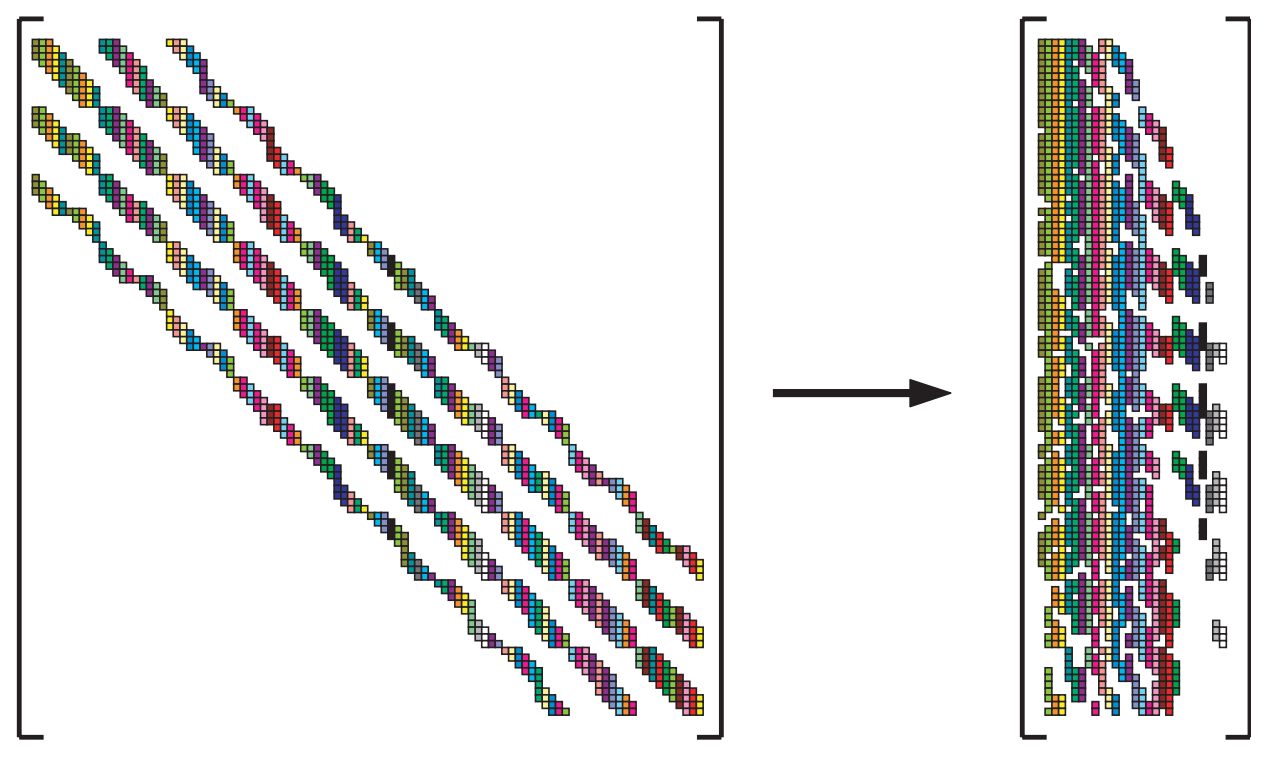
\includegraphics[width=0.8\textwidth]{figures/matrix-compression.png}
  \caption{An example of an efficient Jacobian matrix partitioning \cite{gebremedhin2005color}} \label{fig:matrix-partitioning-example}
\end{figure}


\begin{figure}[htpb]
  \centering
  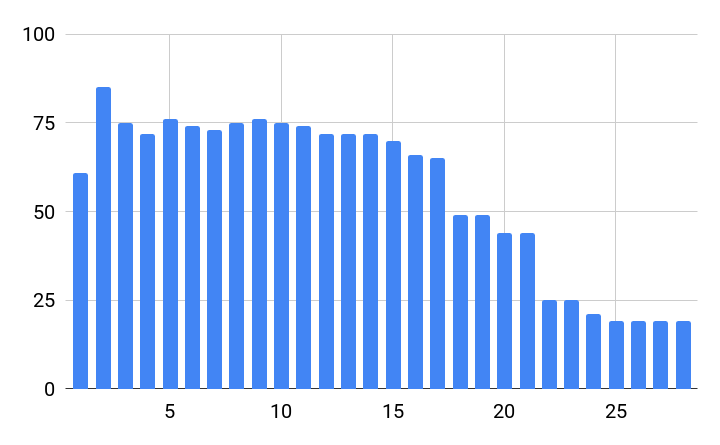
\includegraphics[width=0.8\textwidth]{figures/matrix-compression-2.png}
  \caption{Column length distribution of the example of Figure \ref{fig:matrix-partitioning-example}} \label{fig:matrix-column-distribution}
\end{figure}


According to the ATHLET-NuT coupling design, each column, Figure \ref{fig:matrix-column-distribution}, is transfered to NuT by means of synchronous 3-way handshake procedure, described in Section \ref{sec:athlet-nut-coupling}, right after its evaluation. Thus, Figure \ref{fig:matrix-column-distribution} determines the communication pattern during the Jacobian matrix transfer.\\


% listing
Listing BRA represents a pseudo-code of the current implementation of the compressed Jacobian transfer between ATHLET and NuT. We use this code as a baseline for our following study.\\






%The effect of color size reduction is the particularly field of interest in this study because it determines the communication pattern between the client and server. It is well known that sending small messages can lead to performance deterioration due to not full resource utilization. In this case we consider the network bandwidth as the main resource.\\

%\emph{example of jacobian evaluation}


 

% and there exist several algorithms which can tackle it, namely: [reference to the book]

%The coloring technique 
